\documentclass[12pt,a4paper]{article}
\usepackage{amsmath,amscd,amsbsy,amssymb,latexsym,url,bm,amsthm}
\usepackage{epsfig,graphicx,subfigure}
\usepackage{enumitem,balance}
\usepackage{wrapfig}
\usepackage{mathrsfs,euscript}
\usepackage[usenames]{xcolor}
\usepackage{hyperref}
\usepackage[vlined,ruled,linesnumbered]{algorithm2e}
\usepackage{float}
\hypersetup{colorlinks=true,linkcolor=black}

\newtheorem{theorem}{Theorem}
\newtheorem{lemma}[theorem]{Lemma}
\newtheorem{proposition}[theorem]{Proposition}
\newtheorem{corollary}[theorem]{Corollary}
\newtheorem{exercise}{Exercise}
\newtheorem*{solution}{Solution}
\newtheorem{definition}{Definition}
\theoremstyle{definition}

\renewcommand{\thefootnote}{\fnsymbol{footnote}}

\newcommand{\postscript}[2]
{\setlength{\epsfxsize}{#2\hsize}
	\centerline{\epsfbox{#1}}}

\renewcommand{\baselinestretch}{1.0}

\setlength{\oddsidemargin}{-0.365in}
\setlength{\evensidemargin}{-0.365in}
\setlength{\topmargin}{-0.3in}
\setlength{\headheight}{0in}
\setlength{\headsep}{0in}
\setlength{\textheight}{10.1in}
\setlength{\textwidth}{7in}
\makeatletter \renewenvironment{proof}[1][Proof] {\par\pushQED{\qed}\normalfont\topsep6\p@\@plus6\p@\relax\trivlist\item[\hskip\labelsep\bfseries#1\@addpunct{.}]\ignorespaces}{\popQED\endtrivlist\@endpefalse} \makeatother
\makeatletter
\renewenvironment{solution}[1][Solution] {\par\pushQED{\qed}\normalfont\topsep6\p@\@plus6\p@\relax\trivlist\item[\hskip\labelsep\bfseries#1\@addpunct{.}]\ignorespaces}{\popQED\endtrivlist\@endpefalse} \makeatother

\begin{document}
	\noindent
	
	%========================================================================
	\noindent\framebox[\linewidth]{\shortstack[c]{
			\Large{\textbf{Lab05-DynamicProgramming}}\vspace{1mm}\\
			CS214-Algorithm and Complexity, Xiaofeng Gao, Spring 2021.}}
	\begin{center}
		\footnotesize{\color{red}$*$ If there is any problem, please contact TA Haolin Zhou.}
		
		% Please write down your name, student id and email.
		\footnotesize{\color{blue}$*$ Name:\underline{Xin Xu}  \quad Student ID:\underline{519021910726} \quad Email: \underline{xuxin20010203@sjtu.edu.cn}}
		
	\end{center}
	
	\begin{enumerate}
		\item \textit{Optimal Binary Search Tree.} Given a sorted sequence $K=\left \langle k_{1}, k_{2}, \ldots, k_{n} \right \rangle$ of $n$ distinct keys, and we wish to build a binary search tree from these keys. For each key $k_{i}$, we have a probability $p_{i}$ that a search will be for $k_{i}$. Some searches may be for values not in $K,$ and so we also have $n+1$ \emph{dummy keys} $d_{0}, d_{1}, d_{2}, \ldots, d_{n}$ representing values not in $K$. In particular, $d_{0}$ represents all values less than $k_{1}$, and $d_{n}$ represents all values greater than $k_{n}$. For $i=1,2, \ldots, n-1,$ the dummy key $d_{i}$ represents all values between $k_{i}$ and $k_{i+1}$. For each dummy key $d_{i}$, we have a probability $q_{i}$ that a search will correspond to $d_{i}$. Each key $k_{i}$ is an internal node, and each dummy key $d_{i}$ is a leaf. Every search is either successful (finding some key $k_{i}$ ) or unsuccessful (finding some dummy key $d_{i}$ ), and so we have $ \sum_{i=1}^{n} p_{i}+\sum_{i=0}^{n} q_{i}=1 $. 
		\begin{enumerate}
			\item Prove that if an optimal binary search tree $T$ ($ T $ has the smallest expected search cost) has a subtree $T^{\prime}$ containing keys $k_{i}, \ldots, k_{j},$ then this subtree $T^{\prime}$ must be optimal as well for the subproblem with keys $k_{i}, \ldots, k_{j}$ and dummy keys $d_{i-1}, \ldots, d_{j}$. 
			\item We define $e[i, j]$ as the expected cost of searching an optimal binary search tree containing the keys $k_{i}, \ldots, k_{j} .$ Our goal is to compute $e[1, n]$. Write the state transition equation and pseudocode using \textbf{dynamic programming} to find
			the minimum expected cost of a search in a given binary tree. (\textbf{Remark}: You may use $ w(i, j)=\sum_{l=i}^{j} p_{l}+\sum_{l=i-1}^{j} q_{l} $).
			\item Implement your proposed algorithm in C/C++ and analyze the time complexity. ({\color{blue}The framework Code-OBST.cpp is attached on the course webpage}). Give the minimum search cost calculated by your algorithm. The test case is given as following:
			\begin{table}[H]
				\setlength{\abovecaptionskip}{0cm}
				\setlength{\belowcaptionskip}{0.1cm}
				\centering		
				\begin{tabular}{|c|cccccccc|}
					\hline
					$ i $&0&1&2&3&4&5&6&7\\
					\hline
					$ p_{i} $&&0.04&0.06&0.08&0.02&0.10&0.12&0.14\\
					\hline
					$ q_{i} $&0.06&0.06&0.06&0.06&0.05&0.05&0.05&0.05\\
					\hline
				\end{tabular}
			\end{table}
			\item Please draw the structure of the optimal binary search tree in the test case, and explain the drawing process.   
		\end{enumerate}
		    \begin{solution}
		        \begin{enumerate}
					\item 
					\begin{proof}
					        We can prove it by contradiction. If an optimal binary search tree $T$ has a subtree $T'$ which is not optimal, then we can contruct an optimal subtree $T^*$ and replace $T'$ by $T^*$. And this replacement doesn't change the output of the research but results in a better performance. So the tree $T$ is not optimal, and our hypothesis is wrong.
							Thus everysubtree of an optimal binary tree is optimal.
					\end{proof}
					\item With the definition of $e[i, j]$ and $w(i, j)$ and the conclusion of \textbf{problem (a).}, the recursive equation of $e[i,j]$ can be defined as:
					      \\$e[i,j]=w(i,j)+min(e[i,k-1]+e[k+1,j]),i\leqslant k\leqslant j, \text{and } e[i,j]=0 \text{ for any integer }i>j.$
						  \\ \begin{algorithm}[H]
							\KwIn{a sorted sequence $K=<k_1,k_2,k_3,\ldots ,k_n>$, and the probability $P$ of $K$ that $P=<p_1,p_2,p_3,\ldots,p_n>$ plus the probability of dummy keys $Q=<q_1,q_2,q_3,\ldots,q_n>$.}
							\KwOut{Optimal binary search tree and minimum cost.}
							
							\BlankLine
							\caption{Optimal Binary Search Tree}\label{Alg-OBST}
				
							\For{$i= 1$ \KwTo $n$}{
								\For{$j=i$ \KwTo $n$}{
									compute $w(i,j), w(i, j)=\sum_{l=i}^{j} p_{l}+\sum_{l=i-1}^{j} q_{l} $\;	
								}
							}
							\For{$i=0$ \KwTo $n-1$}{
								\For{$j=1$ \KwTo $n-i$}{
									$e[j,j+i]=w(j,j+i)+min_{j\leqslant k\leqslant j+i}(e[j,k-1]+e[k+1,j+i])$\;
								}
							}

							
							Output $e[1,n]$;
			
						\end{algorithm}
					\item The time complexity to compute $w(i,j)$ is $O(n^3)$. The time complexity to compute $e[i][j]$ is $O(n^3)$, too. The time complexity to construct an optimal binary search tree is $O(n\log n)$ according to the conclusion of recursive tree. So, the total time complexity of OBST is $O(n^3)$.
					And the minimum search cost calculated by my algorithm is $2.68$.
					\item Everytime the function print\_tree print the root of given range and invokes itself recursively. There is a bool parameter to determine whether the print one is the left child or right child. when the range is illegal, we print dummy key $d_i$ as the return state. The structure of the optimal binary search tree is below.
					\\\begin{figure}[htbp]
						\centering
						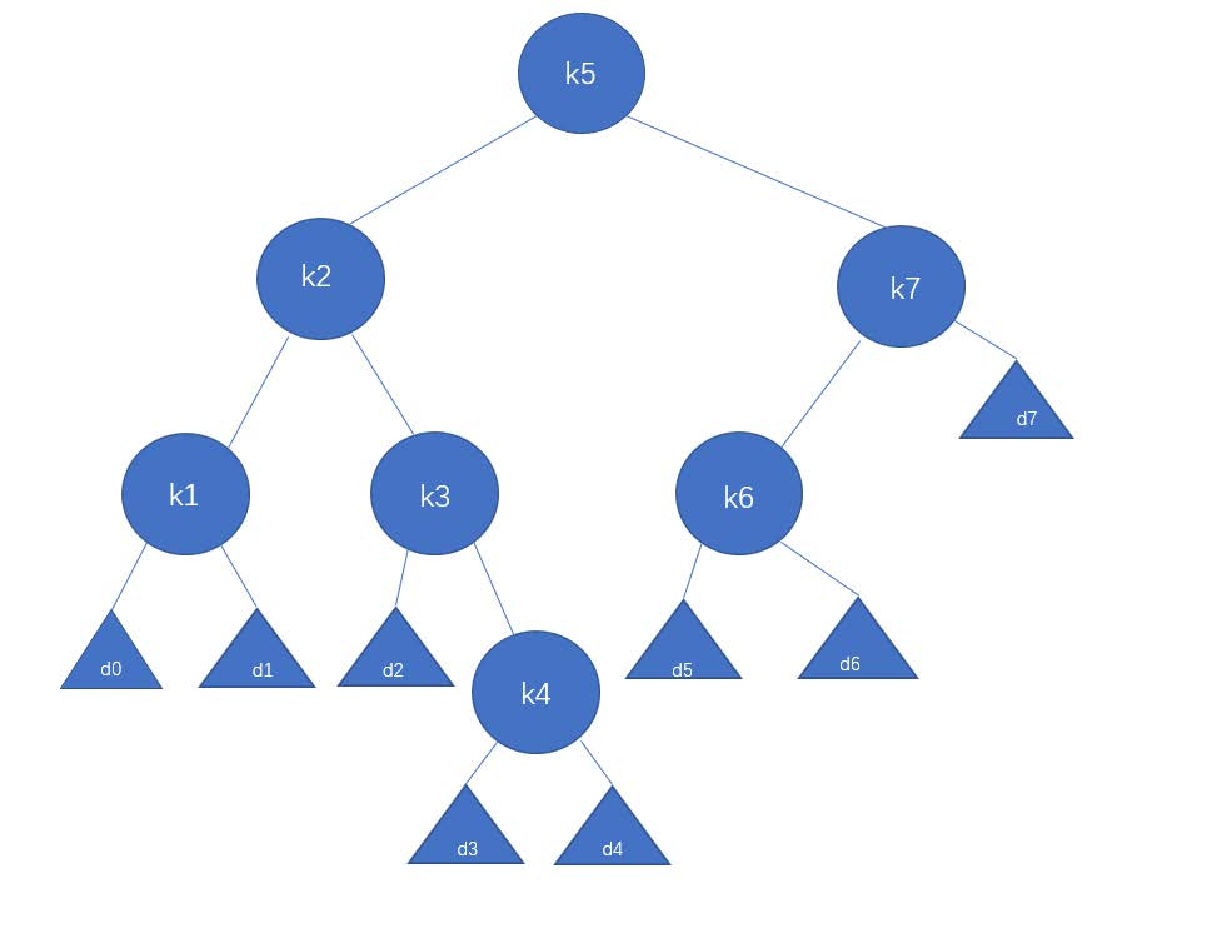
\includegraphics[width=0.4\textwidth]{OBST.pdf}
						\caption{The Optimal Binary Search Tree}\label{OBST}
					\end{figure}
				\end{enumerate}
		    \end{solution}
		
		\item \textit{Dynamic Time Warping Distance.} \textbf{DTW} stretches the series along the time axis in a dynamic way over different
		portions to enable more effective matching. Let $D T W(i, j)$ be the optimal distance between the first $i$ and first $j$ elements of two time series $\bar{X}=\left(x_{1} \ldots x_{n}\right)$ and $\bar{Y}=\left(y_{1} \ldots y_{m}\right),$ respectively. Note that the two time series are of lengths $n$ and $m$, which may not be the same. Then, the value of $D T W(i, j)$ is defined recursively as follows:
		$$
		DTW(i, j)=\left|x_{i}- y_{j}\right|+\min(DTW(i, j-1), DTW(i-1, j), DTW(i-1, j-1))
		$$
		
		\begin{enumerate}
			\item Implement the proposed DTW algorithm in C/C++ and analyze the time complexity of your implementation. ({\color{blue}The framework Code-DTW.cpp is attached on the course webpage}). Two test cases have been given in the source code. 
			\item The window constraint imposes a minimum level $w$ of positional alignment between matched elements. The window constraint requires that $DTW(i, j)$ be computed only when $|i-j| \leq w$. Modify your code to add a window constraint and give the results of $ w=0 $ and $ w=1 $ on the two test cases. 
		\end{enumerate}
		    \begin{solution}
		        \begin{enumerate}
					\item The time complexity to initiate $DTW[i][j]$ is $O(mn)$. The time to find the path is $O(m+n)$. The time to calculate the time normalized distance is $O(m+n)$ too. So, the total time complexity is $O(mn)$.
					\item The .cpp file is in the folder. There are some mistakes in it, but I really don't know how to correct it.
				\end{enumerate}
		    \end{solution}
		
	\end{enumerate}
	
	\vspace{20pt}
	
	\textbf{Remark:} You need to include your .pdf and .tex and {\color{red}\emph{$2$}} source code files in your uploaded .rar or .zip file. Screenshots of test case results are acceptable.
	
	%========================================================================
\end{document}
